% Manuscript source — Astronomy and Computing (Elsevier).
\documentclass[preprint,12pt]{elsarticle}

\usepackage{graphicx}
\usepackage{amsmath}
\usepackage[english]{babel}
\usepackage[protrusion=true,expansion=false]{microtype}

\setlength{\emergencystretch}{2em}
\hyphenpenalty=800
\exhyphenpenalty=800
\journal{Astronomy and Computing}

\begin{document}

\begin{frontmatter}

\title{A Reproducible Control-Validation Workflow for Circular-Shift and
Surrogate Tests of Galactic Radial Profiles}


\author[aff1]{Vitor M. F. Figueiredo\corref{cor1}}
\ead[url]{https://orcid.org/0009-0004-7358-4622}
\cortext[cor1]{Corresponding author.}
\address[aff1]{Independent Researcher, Nisa, Portugal}

\begin{abstract}
\begin{sloppypar}
Correlations between radially organized covariates and the residuals of
galaxy rotation-curve fits are used as diagnostics of inner-region
structure. Assessing such correlations requires controls that account for
the strong radial organization of the underlying data, because a
correlation can exceed a simple label-shuffle comparison while reflecting
only a broad, smooth radial trend. We present a reproducible,
branch-separated control-validation workflow for radial-structure
diagnostics in SPARC-like rotation-curve data. For a partial-rank branch
of 134 galaxies, a radius-conditioned partial-rank statistic is compared
against stochastic shuffle/permutation empirical control distributions and
against exact circular-shift randomization distributions that preserve
radial ordering. The observed absolute partial-rank statistic has
across-galaxy median $\simeq 0.509$; the shuffle control
median-of-medians is $\simeq 0.182$, whereas the ordering-preserving exact
circular-shift control median-of-medians is $\simeq 0.532$, comparable to
the observed statistic. For a separate spectral-control branch of 76
galaxies, an amplitude-based spectral-concentration statistic is evaluated
against amplitude-preserving random-phase controls; because the statistic
is amplitude-based, equality with these controls holds by construction and
is reported as a caveat rather than as evidence. Fixed smooth profiles are
included as deterministic comparators, not stochastic controls. We
document the workflow, its deterministic-seed implementation, and an
audited descriptive demonstration for reuse, and make no physical
interpretation or model-validation claim.
\end{sloppypar}
\end{abstract}

\begin{keyword}
methods: statistical \sep methods: data analysis \sep galaxies: kinematics
and dynamics \sep surrogate data \sep permutation testing \sep
reproducibility
\end{keyword}

\end{frontmatter}

% Purpose: motivate control validation for radial-structure diagnostics and state the contribution.
\section{Introduction}
\label{sec:introduction}

Radial-structure diagnostics correlate a radially organized covariate with
the residuals of galaxy rotation-curve fits in order to probe inner-region
structure. Rotation curves and radial profiles are widely used observational
diagnostics in galaxy studies, including broad rotation-curve reviews,
high-resolution nearby-galaxy rotation-curve surveys, and galaxy-mass reviews
\citep{SofueRubin2001,deBlok2008,Courteau2014}. A practical difficulty is
that the radius itself, and any smooth radially organized covariate, can
induce apparent correlations that do not reflect localized structure. Establishing
whether a measured correlation
carries information beyond broad radial organization is therefore primarily
a computational and statistical problem of control design.

Permutation and surrogate procedures are established tools in general
statistical and correlation-testing contexts, with related resampling and
non-parametric methods widely discussed in astronomy-statistics practice
\citep{SchreiberSchmitz2000,Lancaster2018,FeigelsonBabu2012,PhipsonSmyth2010,YuHutson2022}.
They also have a lineage in surrogate-data testing of an observed statistic
against randomized alternatives \citep{Theiler1992}. These procedures are
general-purpose; we
do not claim that any particular control family is common published
practice in rotation-curve analysis. Different control families preserve
different structure, and a correlation that exceeds a label-shuffle
comparison may still be reproduced by controls that preserve radial
ordering.

{\setlength{\emergencystretch}{2em}
In this work we present a reproducible, branch-separated control-validation
workflow for radial-structure diagnostics in SPARC-like rotation-curve data
\citep{Lelli2016}. The implemented workflow is referred to here as the Nisa
Radial Control Battery (NRCB). The workflow evaluates a radius-conditioned
partial-rank statistic against stochastic shuffle/permutation empirical control
distributions and against exact circular-shift randomization distributions,
and evaluates an amplitude-based spectral-concentration statistic against
amplitude-preserving random-phase controls and fixed smooth references. Our
contribution is the design of this control battery, its deterministic-seed
implementation, and an audited descriptive demonstration on two explicitly
separated galaxy samples. We make no physical interpretation or
model-validation claim; the demonstration characterizes how the control
families behave, not the astrophysics of any galaxy.
\par}

The paper is organized as follows. Section~\ref{sec:data} defines the data
context and the two sample branches. Section~\ref{sec:methods} defines the
diagnostic statistics and control families. Section~\ref{sec:demonstration}
presents the descriptive demonstration. Section~\ref{sec:discussion} states
limitations, Section~\ref{sec:reproducibility} documents reproducibility,
and Section~\ref{sec:conclusion} concludes.





\section{Data and branch definition}
\label{sec:data}

SPARC provides the rotation-curve data context and comprises 175 galaxies
\citep{Lelli2016}. The computational workflow uses two explicitly separated
samples: an $N=134$ partial-rank branch and an $N=76$ spectral-control branch.
The branch sizes are not interchangeable.

\subsection{Branch membership}

The frozen partial-rank branch required completion of the reconstruction
contract with at least eight valid radii, finite required vectors, positive
radial and velocity fields, a finite radial-template covariate, and a
computable radius-conditioned statistic. The statistic-level implementation
separately requires at least five finite joint points.

The spectral-control branch is the subset with at least 16 reconstructed
points, at least 16 finite unique positive-radius samples, finite interpolation
to a fixed 64-point log-radius grid, and nonzero finite spectral power.

The radius-conditioning coordinate is the dimensionless observed-radius
fraction
\begin{equation}
r_{gi}=\frac{R_{gi}}{R_{\max,g}},
\qquad
R_{\max,g}=\max_i R_{gi},
\end{equation}
where $R_{gi}$ is taken from the observed rotation-curve radius column after
nonfinite or nonpositive radius and velocity rows have been excluded, and
$R_{\max,g}$ is the maximum retained observed radius for galaxy $g$. The same
coordinate is used in the post-reconstruction validity mask and partial-rank
residualization. Correctly constructed values lie in $0<r_{gi}\leq1$. The
adapter also applies a permissive upper check $r_{gi}\leq1.1$; this check is a
post-construction implementation guard and does not redefine the
normalization or admit any additional correctly constructed observed-radius
fraction.


\section{Methods}
\label{sec:methods}

\subsection{Diagnostic definitions}
\label{sec:diagnostics}

For galaxy $g$, let $i=1,\ldots,n_g$ index its frozen valid radial bins. Let
$r_{gi}$ denote the radius-conditioning coordinate,
$y_{gi}=|\log_{10}(v_{\mathrm{rec},gi}/v_{\mathrm{obs},gi})|$ the residual
magnitude, and $\sigma_{gi}$ the reconstructed total radial covariate.

\subsubsection{Radial-template covariate and partial-rank statistic}

The normalized covariate and radial-template function are
\begin{equation}
c_{gi} =
\frac{\sigma_{gi}}
{\operatorname{median}\{\sigma_{gj}:\sigma_{gj}>0,\ \sigma_{gj}\ {\rm finite}\}},
\end{equation}
and
\begin{equation}
t(c)=\operatorname{clip}_{[0,1]}
\left[
\exp\left\{-\left(\frac{\log_{10}(\max(c,10^{-12}))}{0.50}\right)^2\right\}
\right].
\end{equation}
A scale fallback of one is used when no finite positive covariate value
exists, and nonfinite normalized entries are replaced by zero.

Let $\operatorname{rank}(\cdot)$ assign average ranks to ties and
$X_g=[\mathbf{1},\operatorname{rank}(r_g)]$. For any vector $z_g$, define
\begin{equation}
\widehat{\beta}_z=\underset{\beta}{\arg\min}\,
\|\operatorname{rank}(z_g)-X_g\beta\|_2^2,\qquad
u_z=\operatorname{rank}(z_g)-X_g\widehat{\beta}_z,
\end{equation}
implemented through least-squares fitting. The signed statistic is
\begin{equation}
\rho_g=\operatorname{corr}\left(u_{t(c)},u_y\right),
\end{equation}
and the production-facing headline summary uses $|\rho_g|$.

\subsubsection{Spectral concentration}

Each valid profile is linearly interpolated onto 64 evenly spaced points in
$\log_{10}(R/\operatorname{median}_{+}(R))$ and mean-centered. After a
real-valued Fourier transform and removal of the DC component, define
\begin{equation}
p_k=\frac{|F_k|^2}{\sum_j |F_j|^2},
\qquad
C=1-\frac{-\sum_k p_k\log p_k}{\log K},
\end{equation}
where $K$ is the number of retained non-DC power bins.

\subsection{Control families and empirical summaries}
\label{sec:controls}

Permutation and surrogate procedures are established tools in general
statistical and correlation-testing contexts
\citep{SchreiberSchmitz2000,PhipsonSmyth2010,YuHutson2022}.

\subsubsection{Shuffle/permutation controls}

For each partial-branch galaxy, $M=1000$ deterministic-seed realizations
permute only the normalized radial covariate. Radius and residual vectors
remain frozen, and the template function is applied after permutation. This
general baseline does not imply common practice in rotation-curve analysis.

\subsubsection{Exact circular-shift randomization distributions}

For a galaxy with $n_g$ valid bins, the production-facing
ordering-preserving control uses every offset in
\begin{equation}
\mathcal{S}_g=\{1,2,\ldots,n_g-1\}
\end{equation}
exactly once. Offset zero is excluded. For each $s\in\mathcal{S}_g$,
$c_g^{(s)}=\operatorname{roll}(c_g,s)$ is transformed and evaluated with the
same radius-conditioned statistic.

Cyclic wrap-around is an operational finite-sample randomization convention,
not a claim that the innermost and outermost radial bins are physically
adjacent. Only the normalized radial covariate is rolled; the radius vector,
residual profile, finite sample size, and frozen validity mask remain fixed.
Applying every non-identity offset preserves the ordered covariate sequence
under translation and defines an exact finite randomization space over all
nontrivial cyclic alignments. The comparison tests sensitivity to radial
ordering and alignment between the radial-template covariate and residual
profile, conditional on this operational convention.

\subsubsection{Amplitude-preserving random-phase controls}

For each spectral-valid residual and radial-template profile, $M=1000$
controls preserve Fourier amplitudes while randomizing the unconstrained
phases at positive frequencies. The mean-centered DC component is zero; the
even-length Nyquist coefficient remains real with a randomized sign; and an
inverse real-valued Fourier transform restores the profile
\citep{Theiler1992,SchreiberSchmitz2000}. More constrained surrogate families
can preserve additional data properties \citep{SchreiberSchmitz1996}, but the
present random-phase tier is intentionally limited to amplitude preservation
and is interpreted only within that control-family definition.

The random-phase comparison is included as a sensitivity diagnostic for the
spectral statistic: because spectral concentration is amplitude-based,
amplitude-preserving phase randomization demonstrates which quantities are
invariant by construction rather than providing independent physical
evidence.

\subsubsection{Smooth fixed references}

On a 64-point coordinate $x\in[0,1]$, the fixed profiles are
\begin{equation}
\exp(-x),\qquad \max(1-x,0),\qquad \max(1-x,0)^2.
\end{equation}
They are fixed references, not stochastic controls, and receive no empirical
percentile or p-value.

\subsubsection{Empirical summaries}

For finite observed value $z_{\rm obs}$, finite controls
$\{z_m\}_{m=1}^{M_v}$, and $\epsilon=10^{-12}$, define
\begin{equation}
L=\#\{z_m<z_{\rm obs}-\epsilon\},\quad
E=\#\{|z_m-z_{\rm obs}|\leq\epsilon\},\quad
G=\#\{z_m>z_{\rm obs}+\epsilon\},
\end{equation}
with $L+E+G=M_v$. The bounded mid-rank percentile is
\begin{equation}
q=\operatorname{clip}_{[0,1]}\left(\frac{L+E/2}{M_v}\right).
\end{equation}
For signed or absolute random-tier statistics,
\begin{equation}
p_{\rm MC}=\operatorname{clip}_{[0,1]}
\left[
\frac{1+\#\{|z_m|\geq |z_{\rm obs}|-\epsilon\}}{M_v+1}
\right].
\end{equation}
The same formula is used for the exhaustive nontrivial circular-shift set.
For the nonnegative phase-blind spectral statistic,
$p_{\rm spectral}=\min\{1,2\min(q,1-q)\}$. Fixed references receive neither
an empirical percentile nor an empirical p-value.



\section{Demonstration}
\label{sec:demonstration}

Figure~\ref{fig:workflow} presents the branch-separated computational
workflow. Shuffle/permutation controls define stochastic empirical control
distributions. Circular-shift controls instead use exhaustive nontrivial
radial offsets to define exact circular-shift randomization distributions.

\begin{figure}[htbp]
  \centering
  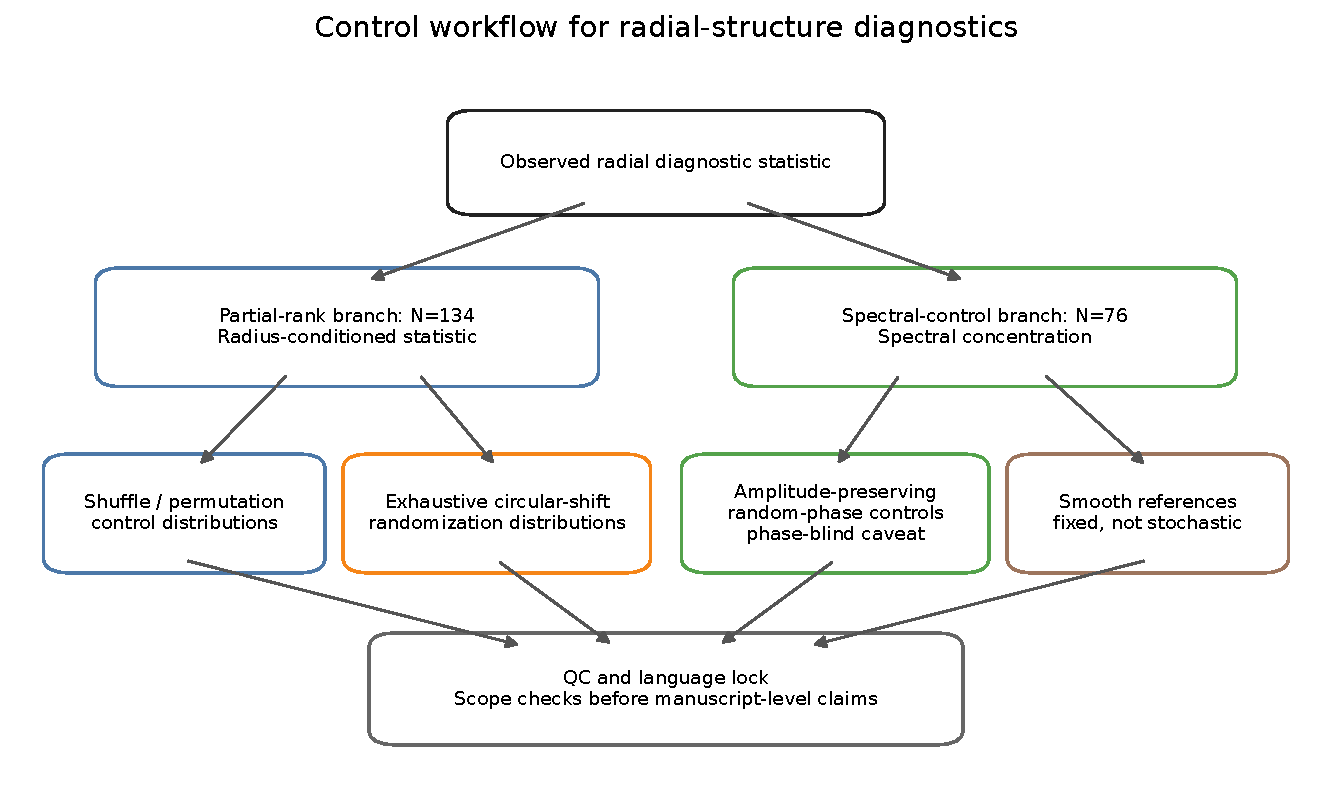
\includegraphics[width=\linewidth]{../figures/figure1_workflow_control_validation_rev1.pdf}
  \caption{Control workflow for radial-structure diagnostics. The workflow
  separates the $N=134$ partial-rank branch from the $N=76$ spectral-control
  branch. Shuffle/permutation controls form stochastic empirical control
  distributions, whereas circular-shift controls use exhaustive nontrivial
  radial offsets to define exact circular-shift randomization distributions.
  Amplitude-preserving random-phase controls carry a phase-blind/by-construction
  caveat. Smooth profiles are fixed references, not stochastic controls.}
  \label{fig:workflow}
\end{figure}

For the $N=134$ partial-rank branch, the observed absolute statistic has
median $\simeq0.509$ (IQR $0.280$--$0.773$). Per-galaxy shuffle-control
medians have median $\simeq0.182$ (IQR $0.135$--$0.232$), while exact
circular-shift medians have median $\simeq0.532$ (IQR $0.340$--$0.649$).
Across galaxies, the corresponding empirical p-values have medians
$\simeq0.026$ and $0.500$, respectively. These summaries are not
pooled-across-galaxy p-values.

For the separate $N=76$ spectral branch, residual and radial-template spectral
concentrations have medians $\simeq0.676$ (IQR $0.589$--$0.755$) and
$\simeq0.754$ (IQR $0.663$--$0.817$), respectively. Random-phase control
medians are identical at displayed precision by construction. The
exponential, linear, and quadratic fixed-reference values are approximately
$0.548$, $0.553$, and $0.570$.

\begin{figure}[htbp]
  \centering
  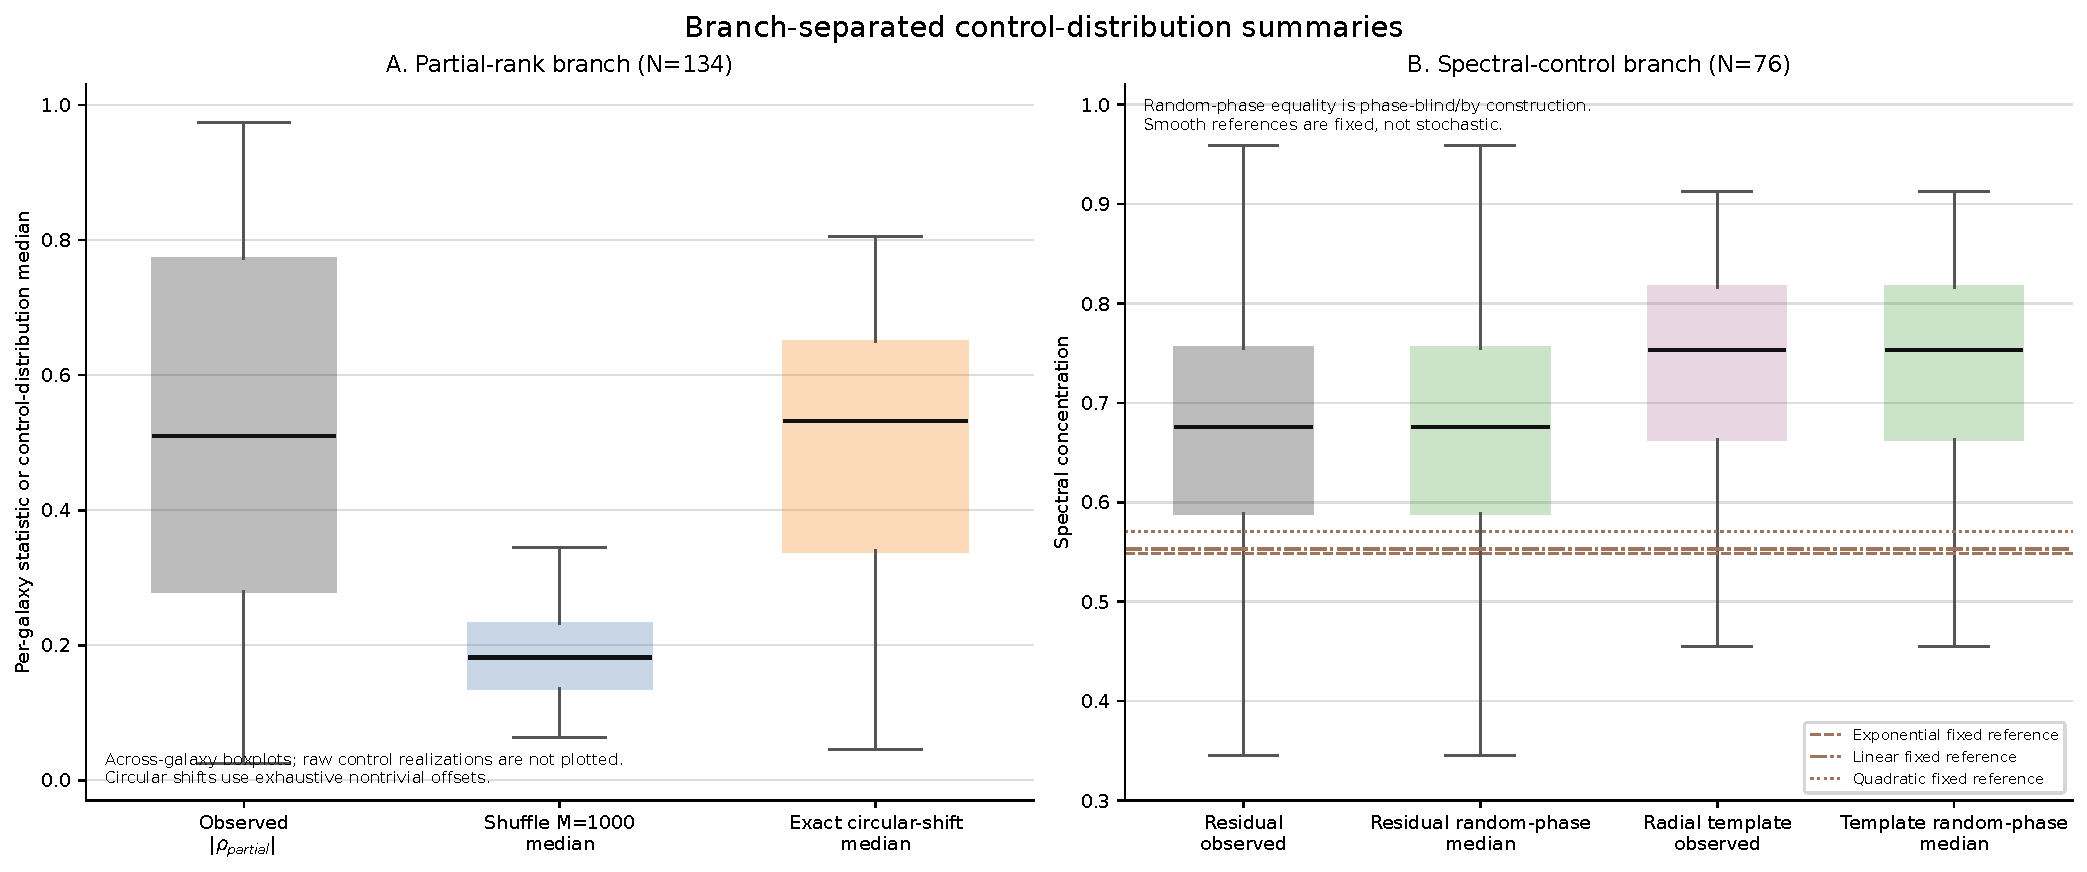
\includegraphics[width=\linewidth]{../figures/figure2_control_distribution_comparison_rev1.pdf}
  \caption{Branch-separated control-distribution summaries. Panel A shows the
  $N=134$ partial-rank branch and per-galaxy medians from the $M=1000$
  shuffle empirical control distributions and exhaustive circular-shift
  randomization distributions. Panel B separately shows the $N=76$
  spectral-control branch, random-phase control medians, and smooth-profile
  fixed references. Panels summarize each per-galaxy control distribution by
  its median; empirical percentiles and p-values remain in the production
  summary table, and the full raw realizations are not plotted. Fixed
  references are not stochastic controls.}
  \label{fig:control-summaries}
\end{figure}

For both spectral targets, per-galaxy mid-rank empirical percentiles are
$0.500$ and doubled equal-tail quantities are $1.000$. This follows from
amplitude preservation and the definition of spectral concentration.

\begin{figure}[htbp]
  \centering
  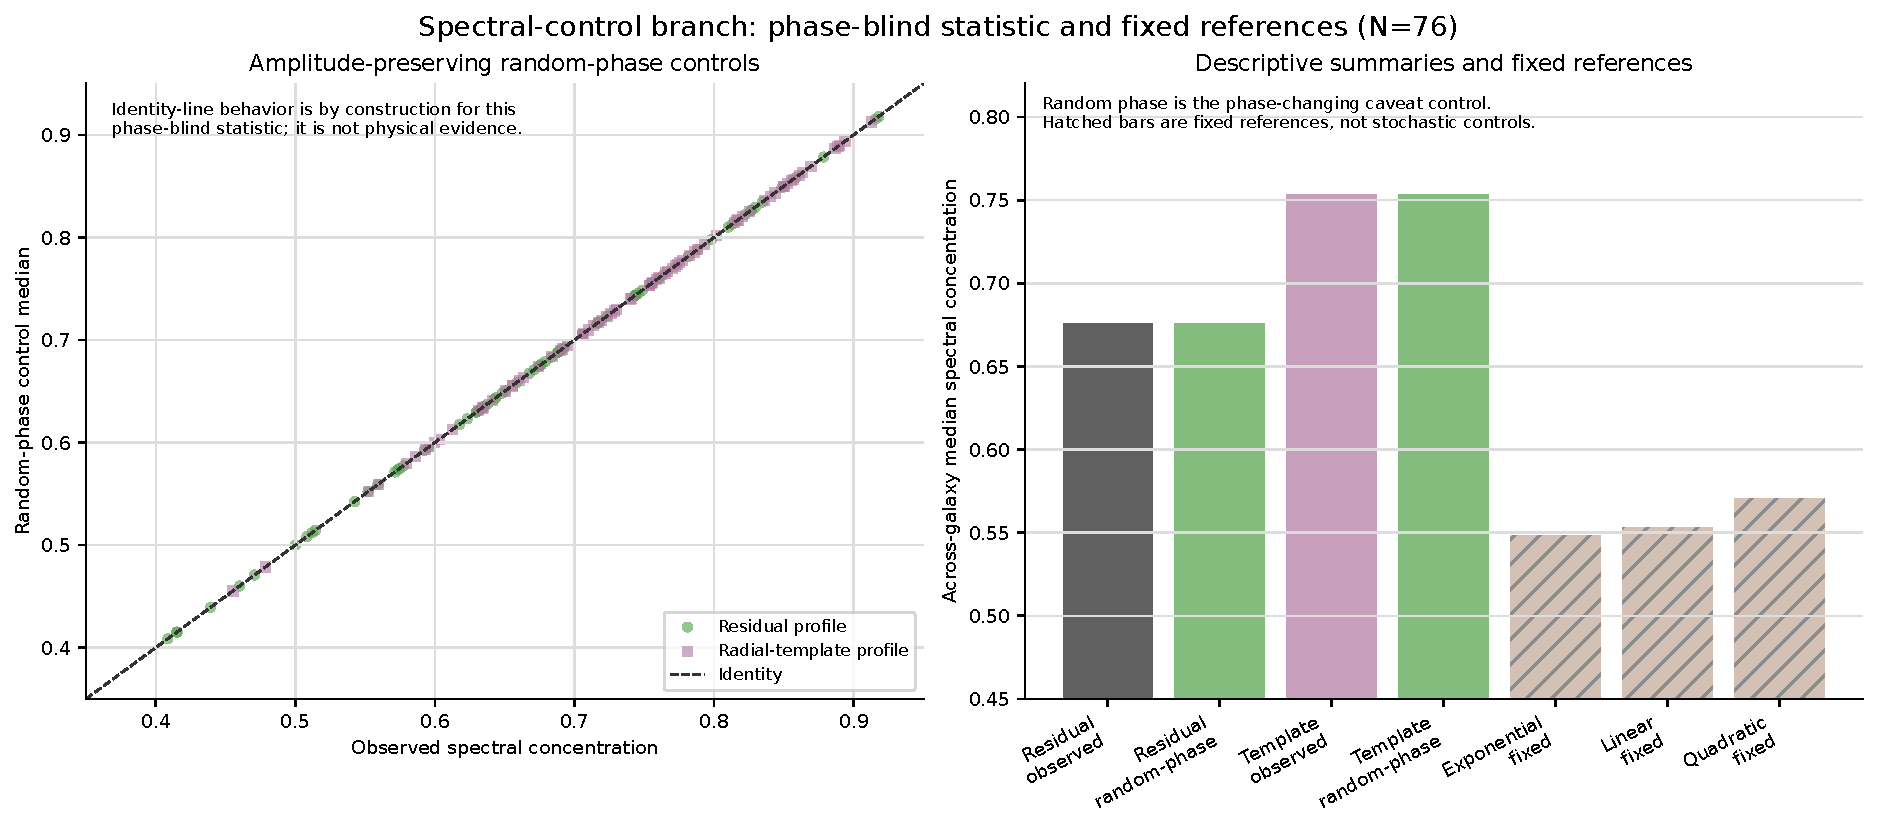
\includegraphics[width=\linewidth]{../figures/figure3_spectral_phase_control_caveat_rev1.pdf}
  \caption{Phase-blind spectral-concentration caveat and fixed references
  ($N=76$). Panel A compares observed spectral concentration with per-galaxy
  medians from amplitude-preserving random-phase controls. Identity-line
  behavior is by construction for the phase-blind statistic and is not
  independent evidence about the profiles. Panel B shows descriptive
  across-galaxy medians; smooth profiles are fixed references, not stochastic
  controls.}
  \label{fig:spectral-caveat}
\end{figure}

% Results redundancy resolved: the descriptive results live in the
% Demonstration section. The former empty Results stub is intentionally
% not included (see notes/FULL_PAPER_MAJOR_REVISION_REPORT.md, Objective 3).

\section{Discussion and limitations}
\label{sec:discussion}

No close rotation-curve or radial-profile control precedent was verified;
the citation scope used here is general-methodological. Cyclic wrap-around is
an operational randomization convention and does not imply physical adjacency
of the radial endpoints. Other defensible designs could include alternative
detrending, residualization against smooth radial profiles, block/permutation
controls, non-cyclic boundary treatments, or alternative radial templates.
These alternatives were not tested here. Random-phase spectral equality is by
construction, smooth profiles are deterministic comparators, and the two
sample branches must remain separated.


\section{Reproducibility}
\label{sec:reproducibility}

The production workflow uses frozen base seed \texttt{20260503} and the exact
seed namespace \texttt{ac-control-validation-m-surrogate-v1}. Randomized seeds
are deterministic unsigned integers derived from the first eight bytes of
SHA256 applied to the namespace, base seed, canonical galaxy name, tier name,
and one-indexed iteration. Python's built-in hash is not used. Circular shifts
and fixed references do not use random seeds.

The release plan follows general scientific-computing and
reproducible-computational-research guidance: record executable entry points,
inputs, outputs, environment details, and provenance sufficient for independent
audit \citep{Wilson2014,Sandve2013}.

The recorded environment includes Python \texttt{3.12.7}, NumPy
\texttt{1.26.4} \citep{Harris2020}, and code commit \texttt{c8a6c950bd9e}. The production entry
point is \texttt{python src/\allowbreak run\_m\_surrogate\_extension.py
\allowbreak --production}.
Invalid realizations were retained and counted in emitted totals while
excluded from valid empirical statistics. Detailed audit records are retained
in repository notes and supplementary provenance files.




% Purpose: summarize the workflow and the descriptive demonstration in one compact section.
\section{Conclusion}
\label{sec:conclusion}

We have presented the Nisa Radial Control Battery (NRCB), a reproducible
control-validation workflow for radial-structure diagnostics in SPARC-like
rotation-curve data. The workflow is branch-separated: a partial-rank branch
of 134 galaxies and a
spectral-control branch of 76 galaxies are analysed independently and are
not interchangeable. By comparing each observed statistic against multiple
control families, the workflow makes explicit how those families behave. A
label-shuffle comparison and an ordering-preserving exact circular-shift
comparison can lead to different conclusions about the same statistic; the
exact circular shifts act as operational finite-sample controls rather than
physical models. For the amplitude-based spectral-concentration statistic,
equality with amplitude-preserving random-phase controls holds by
construction and is reported as a caveat, and fixed smooth profiles are
deterministic comparators rather than stochastic controls.

We make no physical interpretation, discovery, or model-validation claim;
the demonstration is descriptive and characterizes control behavior on the
two samples. Natural methodological extensions include alternative
detrending, non-cyclic boundary conventions, block or permutation controls,
additional radial templates, and application to broader datasets.


% Elsevier requirement: this declaration must appear immediately above the
% references.
\section*{Declaration of generative AI and AI-assisted technologies in the
writing process}
\begin{sloppypar}
During the preparation of this work, the author used OpenAI ChatGPT and Codex, Anthropic Claude and claude code, Google Gemini and Grok for drafting assistance, language refinement, code-review support, and the preparation of audit checklists. After using these tools, the author reviewed and edited the content as needed and takes full responsibility for the content of the publication.
\end{sloppypar}


\bibliographystyle{elsarticle-harv}
\bibliography{references}

\end{document}
